\documentclass[xcolor=x11names,compress]{beamer}
\usepackage[english]{babel}

%% General document %%%%%%%%%%%%%%%%%%%%%%%%%%%%%%%%%%
\usepackage{graphicx}
\usepackage{tikz}
\usepackage{wrapfig}
\usepackage{hyperref,natbib}

\usetikzlibrary{decorations.fractals}
%%%%%%%%%%%%%%%%%%%%%%%%%%%%%%%%%%%%%%%%%%%%%%%%%%%%%%


%% Beamer Layout %%%%%%%%%%%%%%%%%%%%%%%%%%%%%%%%%%
\useoutertheme[subsection=false,shadow]{miniframes}
\useinnertheme{default}
\usefonttheme{serif}
\usepackage{palatino}

\setbeamerfont{title like}{shape=\scshape}
\setbeamerfont{frametitle}{shape=\scshape}

\setbeamercolor*{lower separation line head}{bg=DeepSkyBlue4} 
\setbeamercolor*{normal text}{fg=black,bg=white} 
\setbeamercolor*{alerted text}{fg=red} 
\setbeamercolor*{example text}{fg=black} 
\setbeamercolor*{structure}{fg=black} 
 
\setbeamercolor*{palette tertiary}{fg=black,bg=black!10} 
\setbeamercolor*{palette quaternary}{fg=black,bg=black!10} 

\renewcommand{\(}{\begin{columns}}
\renewcommand{\)}{\end{columns}}
\newcommand{\<}[1]{\begin{column}{#1}}
\renewcommand{\>}{\end{column}}
%%%%%%%%%%%%%%%%%%%%%%%%%%%%%%%%%%%%%%%%%%%%%%%%%%
\newcommand{\hlb}[1]{\textbf{\textcolor{blue}{#1}}}
\newcommand{\hl}[1]{\textcolor{blue}{#1}}
\newcommand{\lien}[2]{\mathcal{L}_{#1}^{#2}}
\newcommand{\lie}[1]{\mathcal{L}_{#1}}

\newcommand{\case}[1]{\textbf{Case #1:}}

%\usepackage[english]{babel}
\usepackage[utf8]{inputenc}
%\usetheme{Goettingen}

\begin{document}
\title{Bifurcations in continuous time piecewise smooth dynamical systems}
\author{Debsankha Manik}

\begin{frame}
\titlepage
\end{frame}

\begin{frame}{A brief summary on PWS flows}
A simple piecewise smooth function:
\begin{displaymath}
   \dot{x} = \left\{
     \begin{array}{lr}
       F_1(x) & : H(x) < 0\\
       F_2(x) & : H(x) >0
     \end{array}
   \right.
\end{displaymath}

Switching manifold: $H(x)=0$

The flows of $F_1$ and $F_2$ are $\varphi_1(x)$ and $\varphi_2(x)$ 
respectively, defined in respective regions and also in the neighbourhood of 
the switching manifold:

\begin{align}
\dot{\varphi_1}&=F_1\\
\dot{\varphi_2}&=F_2
\end{align}
 
\end{frame}

\begin{frame}
\begin{figure}
\caption{Example: Impact Oscillator}
\begin{center}
\includegraphics[width=0.9\columnwidth]{../2011-11-20/osc-pw}
\end{center}
\end{figure}

\end{frame}




\begin{frame}{How to analyze nonlinear systems?}
\begin{figure}
\caption{Look at the vector field}
\begin{center}
\includegraphics[width=0.9\columnwidth]{vfield}
\end{center}
\end{figure}


\end{frame}

\begin{frame}
\begin{figure}
\caption{Possible scenarios}
\begin{center}
\includegraphics[height=0.84\textheight]{../2011-09-11/c-bifs}
\end{center}
\end{figure}

\end{frame}


\section{Bifurcation of equillibria}

\begin{frame}
Choose a coordinate system such that:\\
\begin{displaymath}
   \dot{\bf{x}} = \left\{
     \begin{array}{lr}
       F_1(\bf{x},\mu) & : x_n<0\\
       F_2(\bf{x},\mu) & : x_n>0
     \end{array}
   \right.
\end{displaymath}

and $\bf{x}=0$ is a grazing point.  

$x_n==n$th component of $\bf{x}$.  \\

Locally linearize:
\begin{displaymath}
   \dot{\bf{x}} = \left\{
     \begin{array}{lr}
       \bf{A_1x+\bf{B}\mu} & : x_n<0\\
       \bf{A_2x+\bf{B}\mu} & : x_n<0\\
     \end{array}
   \right.
\end{displaymath}

Where:\\
\[
\bf{A_i}=\left.\frac{\partial F_i}{\partial \bf{x}}\right|_{x=0}
\]
and 
$\bf{B}=\frac{\partial F_1}{\partial \mu}\left.\right|_{\mu=0}=\frac{\partial F_2}{\partial \mu}\left.\right|_{\mu=0}$
 (Due to continuity).

Also, $\bf{A_1}$ and $\bf{A_2}$ can differ only in the $n-$th column (Again due to continuity).


\end{frame}


\begin{frame}
Let:
$A_1\bf{x}^*_1+\bf{B}\mu=0$,
$A_2\bf{x}^*_2+\bf{B}\mu=0$.  


Assuming $A_i$'s are invertible:
\[
\bf{x}^*_i=-\bf{A_i}^{-1}\bf{B}\mu=-\frac{adj(\bf{A_i})}{det(\bf{A_i})}\bf{B}\mu
\]

The solutions exist iff:
\[
x^*_{1_{n<0}}<0, x^*_{2{_n}}>0. 
\]  

Now, 
\[
x^*_{1_k}=\frac{c^*_{1_k}}{det(\bf{A_1})}\mu, x^*_{2_k}=\frac{c^*_{2_k}}{det(\bf{A_2})}
\]

Where, \[
c^*_{i_k}=[-adj(\bf{A_i)B}]_k=[-adj(\bf{A_i)_{kj}B_j}]
\]

Because $A_1$ differs from $A_2$ only in $n-$th column, $adj(A_1)$ and  
$adj(A_2)$ shares a common $n-$th row,  $c^*_{1_n}=c^*_{2_n}:=C$

\end{frame}


\begin{frame}{Condition for border crossing of equillibria}
\[
x^*_{1_n}=\frac{C}{det(\bf{A_1})}\mu, x^*_{2_k}=\frac{C}{det(\bf{A_2})}\mu
\]

{\bf Cases:}\\
\begin{enumerate}
\item $det({\bf A_1})det({\bf A_1})<0$.  $x^*_{1_n}$ and $x^*_{2_n}$ always have 
opposite signs.  \\
\item $det({\bf A_1})det({\bf A_1})>0$.  $x^*_{1_n}$ and $x^*_{2_n}$ always have 
same signs.  
\end{enumerate}

%This result is arrived at \cite{paper:classf-eqbm-bf} by a slight variation  of Feigin's technique. \\
\begin{figure}
\begin{center}
\includegraphics[width=0.9\columnwidth]{../2011-09-11/cases}
\end{center}
\end{figure}

\end{frame}


\begin{frame}{Grazing orbits}
\begin{figure}
\caption{}
\begin{center}
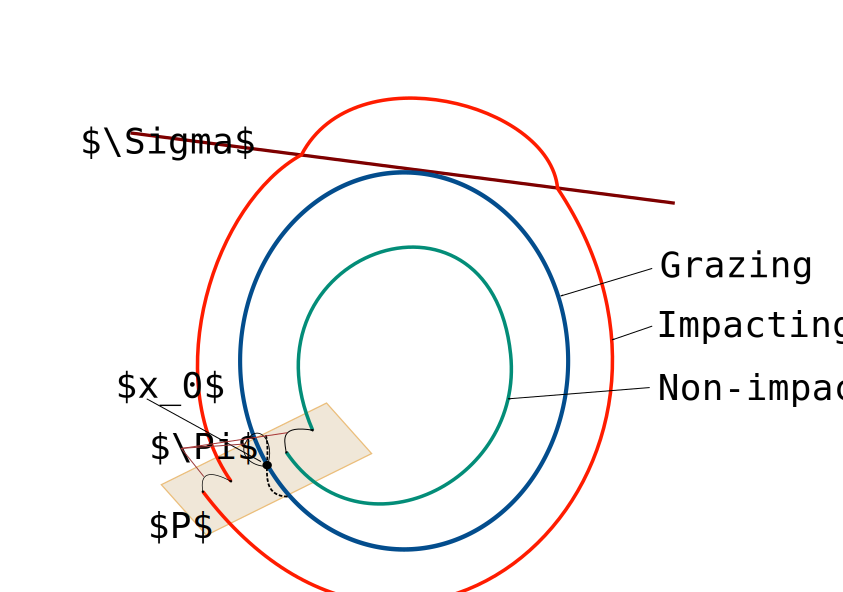
\includegraphics[width=0.9\columnwidth]{../2011-09-19/graz}
\end{center}
\end{figure}


\end{frame}

\begin{frame}{Grazing orbits}
\case{1} $F_1(x)\neq F_2(x)$ at switching manifold:
The Poincare map (given by Nordmak et al\cite{paper:nordmark-sqrt}, using the 
ZDM formalism; also by Molenaar, without ZDM) is of the form:
\begin{align*}
&\left.  \begin{array}{lr}
x_{n+1}=ax_n + y_n + \rho\\
y_{n+1}= -bx_n
\end{array}
\right\}  &x\leq 0\\
&\left.  \begin{array}{lr}
x_{n+1}= -c \sqrt{x_n} + y_n +\rho\\
y_{n+1}= -dx_n
\end{array}
\right\}  & x>0
\end{align*}

\begin{itemize}
\item Jacobian of the system is singular. \\
\item Infinite stretching of the phase space.  \\
\item In some cases, period-adding bifurcation occurs.  \\
\item This singularity affects only the trace of $J$, not the determinant. \cite{paper:sob-trace-sing} 
\end{itemize}

\end{frame}


\begin{frame}

\begin{figure}
\caption{Bifurcation in a map with square root singularity}
\begin{center}
\includegraphics[width=0.9\columnwidth]{../2011-08-14/semi-chao}
\end{center}
\end{figure}
\end{frame}

\begin{frame}
\case{2} $F_1(x)= F_2(x)$ at switching manifold:
The Poincare map (given by Dankowicz and Nordmak ) is of the form:
\begin{align*}
x_{n+1}=\left\{ 
\begin{array}{lr}
ax_n + \rho  &x\leq 0\\
ax_n-bx_n^{3/2}+\rho &x>0
\end{array}
\right.
\end{align*}

\begin{itemize}
\item Jacobian of the system is continuous. \\
\item No chance of border collision bifurcation (Elaborate later).  \\
\item Both trace and determinant of $J$ vary continuously.  
\end{itemize}

\vspace{4em}
\end{frame}


\begin{frame}{Discontinuous Jacobian is necessary for period doubling on BC}

\begin{figure}
\caption{}
\begin{center}
\includegraphics[height=0.4\textheight]{cb}
\end{center}
\end{figure}

Suppose for the parameter value $\mu=0$, the fixed point of the left hand size 
map crosses the boundary $x=0$.  Suppose a period doubling occurs. \\
\end{frame}


\begin{frame}
Now the fixed point of both the maps are at $\delta^2$, say.    
Then: 
\begin{align*}
f_2(f_1(-\epsilon^2))&=-\epsilon^2\\
f_2(\delta^2+\dot{f_1}(\delta^2)(\delta^2+\epsilon^2))&=-\epsilon^2\\
\delta^2+\dot{f_2}(\delta^2)\dot{f_1}(\delta^2)(\delta^2+\epsilon^2))&=-\epsilon^2\\
\dot{f_2}(\delta^2)\dot{f_1}(\delta^2)&=-1\\
\dot{f_2}(0)\dot{f_1}(0)&\approx-1
\end{align*}

Therefore the discontinuity is evident.  
\end{frame}


\begin{frame}{How to understand a border collision bifurcation}
\emph{What do we do in smooth bifurcations?}
\begin{enumerate}
\item Take Poincare section.  
\item Calculate fixed points.  
\item Calculate jacobian and its eigenvalues.  
[If the absolute values of the eigenvalues are $<1$, we will see attractive 
behaviour, otherwise reoulsive.  ]
\end{enumerate}


\emph{What's the problem now?}\\

-There's no easy way to get the Poincare map in a closed form.  \\
\vspace{1em}
\emph{However, we can still compute eigenvalues by searching for a direction 
which remains unchanged in each stroboscopic slice.}
%\footnote{But what if we 
%have damping?  Transient always decays.}\footnote{Does it eliminate the need of 
%Saltation matrix approach?\vspace{1em}}\\

-But we need to find out the fixed points first.  
\end{frame}



\begin{frame}{A border crossing orbit}
\begin{figure}
\caption{}
\begin{center}
\includegraphics[width=0.3\columnwidth]{trajectory}
\end{center}
\end{figure}

Supposing the orbit crosses the border only once.  \\
Then finding out the orbit boils down to:
\begin{align}
x_1&=\varphi_1(x_0,0,\tau_0)\\
H(x_1)&=0\\
x_2&=\varphi_2(x_1,\tau_0,\tau_1)\\
H(x_2)&=0\\
x_0&=\varphi_1(x_2,\tau_1,T-\tau_0-\tau_1)
\end{align}
\end{frame}


\begin{frame}
This is a set of $3n+2$ equations in $3n+2$ unknowns, so this can be tackled 
with standard Newton's method of root finding:\cite{paper:sob-trace-sing}
\[
y_{n+1}=\frac{G(y_n)}{J(\bar{y}_n)}
\]

Here $y:=\left\{x_0,x_1,x_2,\tau_0,\tau_1\right\}$.  

\end{frame}


\begin{frame}{Theory of Border Collision Bifurcations}
For a PWS system, we can now:
\begin{enumerate}
\item Find out all the periodic  orbits.  But finding out a $T_j$ orbit 
involves inverting a $(2j+1)n+2*j$ dimensional matrix.  Since best known 
matrix inversion algorithms are $O(n^2)$, it may not be feasible to do this 
for orbits that cross the border many times.  
\pause{}
\item Then we can find out the eigenvalues of the Poincare map at the fixed 
points by taking small deviations from the periodic orbit and doing a 
least-square style fiting for the parameters for the locally linear map.(Only 
$\delta$ and $\tau$ in case of 2-d)  Interesting phenomena will occur when 
fixed points change nature 
after 
border collision.  

\pause{}
\item Then we apply standard results regarding the stability of fixed learnt in case of 
smooth bifurcations to explain the phenomenon.  
\end{enumerate}

\end{frame}

\begin{frame}
The locally linear map will be, in 2-D:
\[
\begin{bmatrix}
x\\y
\end{bmatrix}	\to\left\{
		\begin{array}{lc}
			\begin{bmatrix}
			\tau_L & 1\\
			-\delta_L & 0
			\end{bmatrix}
				\begin{bmatrix}
				x\\y
				\end{bmatrix} + \mu \begin{bmatrix}
				1\\0
				\end{bmatrix} &x\leq 0
			\\
			\begin{bmatrix}
			\tau_R & 1\\
			-\delta_R & 0
			\end{bmatrix}
				\begin{bmatrix}
				x\\y
				\end{bmatrix}+ \mu \begin{bmatrix}
				1\\0
				\end{bmatrix} &x> 0
		\end{array}
	\right.   
\]

The parameter space of $\left{\delta_L,\delta_R,\tau_L,\tau_R\right}$ can be 
divided into regions exhibiting different behaviours on border collision.  
\cite{paper:classify-pws-bif}
\end{frame}




\begin{frame}
\bibliographystyle{plain}
\bibliography{pws-eqbm}

\end{frame}
\end{document}
